\documentclass[mathserif]{beamer}

\usepackage{pgf}
\usepackage{graphicx}
\usepackage{amsmath}
\usepackage{subfig}
\usetheme{Madrid}
\usecolortheme{seahorse}

\AtBeginSection{
\begin{frame}{Table of Contents}
\tableofcontents[currentsection]
\end{frame}
}

\title[Mesh Movement]{Methods for Mesh Movement and Curved Mesh Generation}
\author[Aditya Kashi]{{\Large Aditya Kashi} \institute[NCSU]{North Carolina State University}}
\date{August 2015}

\bibliographystyle{plain}

\begin{document}
\frame{\titlepage}

\section{Introduction}
\begin{frame}
Various methods have been used to generate high-order curved meshes from linear meshes - including methods to optimize surface (boundary) meshing and methods to get valid internal mesh. Here, I focus on the latter.

There are mainly two classes of methods to achieve mesh movement:
\begin{itemize}
\item Elasticity-based methods
\item Interpolation methods
\end{itemize}
\end{frame}

\section{Elasticity-based Methods}

\begin{frame}{Lineal Spring Analogy}
This is the simplest method that can be used to move internal mesh points in response to movement of the boundary, invented by J.T. Batina (NASA, 1991).

Each edge of the mesh is assumed to represent a lineal spring connecting the two nodes which make up the edge.

The idea is that after imposing boundary movement, the mesh is allowed to ``go to equilibrium". So at every mesh point, we have
\begin{equation}
\sum_j k_{ij}(\Delta \vec{r_i} - \Delta \vec{r_j}) = \vec{0} \quad \forall i
\end{equation}
where $i$ ranges over all nodes, $j$ ranges over points surrounding node $i$ and $\Delta \vec{r_i}$ is the displacement of node $i$.
$k_{ij}$ is the stiffness of the spring between nodes $i$ and $j$, calculated as
\begin{equation}
k_{ij} = \frac{1}{||\vec{r_i} - \vec{r_j}||}
\end{equation}
\end{frame}

\begin{frame}{Lineal Spring Analogy}
It is not reliable as it generates invalid elements (containing zero and negative values of Jacobian determinant).

This method is used, for example, by Mavriplis et. al. \cite{mavriplis}. In this case, however, the internal elements are linear - only boundary faces are high-order, since the problem considered is inviscid flow.
\end{frame}

\begin{frame}{Torsional Spring Analogy}
This is an extension to the previous method, which adds torsional springs at each node in each element. 

\begin{figure}
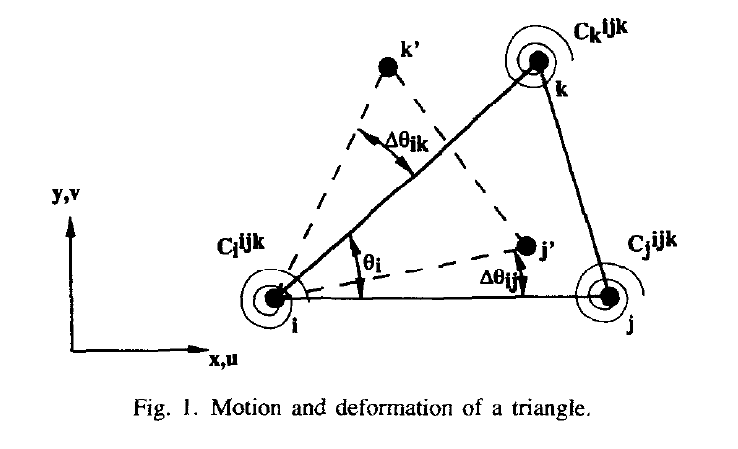
\includegraphics[scale=0.25]{torsionspring}
\end{figure}

These torsional springs resist the relative angular motion between edges of an element. This leads to a substantially more robust movement, according to Farhat et. al. \cite{farhat} However, I have not found any literature (yet) where this method is used for curved mesh generation, though it is widely used for mesh deformation otherwise.
\end{frame}

\begin{frame}{Linear Elasticity Analogy}
In this method, the (partial differential) equations of linear elasticity are solved by high-order continuous FEM to move the internal nodes of a mesh, as done by Xie \cite{xie}.

Even if a constant elasticity is used throughout, it gives decent results. 

But the main power lies in the fact that the elasticity can be varied in a way that leads to a better mesh, such as making it inversely proportional to distance from the deforming boundary, or to the cell volume (as in Hartmann and Leicht \cite{hartmann}) (which I have not done yet).

Idea: A radial basis function could be used to determine the elasticity variation!
\end{frame}

\begin{frame}{Non-linear Elasticity Analogy}
The general idea of this method is same as that of linear elasticity. The difference is that a non-linear constitutive model is used (relating stress and strain) instead of a linear constitutive model. 

Persson and Peraire claim \cite{persson} ``When the mesh is sufficiently fine relative to solid deformation, this method guarantees non-intersecting elements even for highly distorted or anisotropic initial meshes".
\end{frame}

\section{Interpolation Methods}
\begin{frame}
These methods are not based on any physical relation between node locations.

Instead, the boundary displacement is interpolated to the interior using any of several methods.
\end{frame}

\begin{frame}{Delaunay Graph Mapping(DGM)}
Developed by Liu, Qin and Xia \cite{dgm}, this method is a fast method of mesh movement. It consists of the following steps.
\begin{itemize}
\item Triangulate the boundary points of the mesh. This triangulation is referred to as the Delaunay graph.
\item Each internal mesh point is located in the Delaunay graph, and its area coordinates are calculated w.r.t. the Delaunay element it lies in.
\item Using the prescribed boundary displacements, the Delaunay graph is moved.
\item Using the calculated area coordinates, the interior mesh points are mapped back to the deformed Delaunay elements, thus moving the mesh.
\end{itemize}
\end{frame}

\begin{frame}{DGM}

\begin{figure}
	\subfloat{
		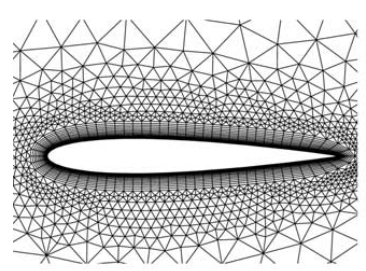
\includegraphics[scale=0.25]{dgm-mesh}
	}
	\subfloat{
		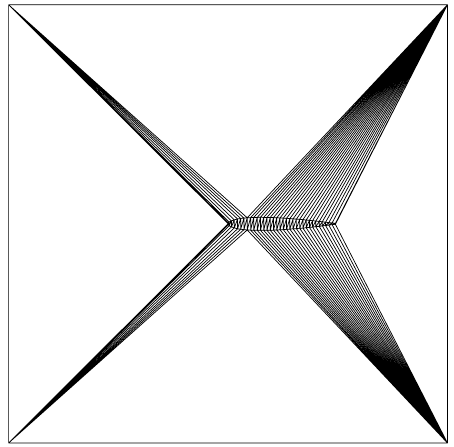
\includegraphics[scale=0.2]{dgm-dg}
	}
	\subfloat{
		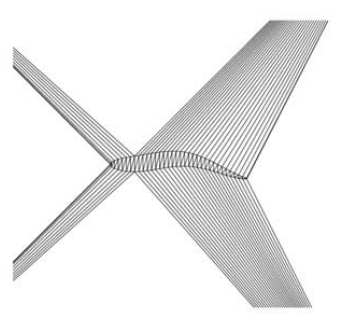
\includegraphics[scale=0.25]{dgm-moveddg}
	}
	\subfloat{
		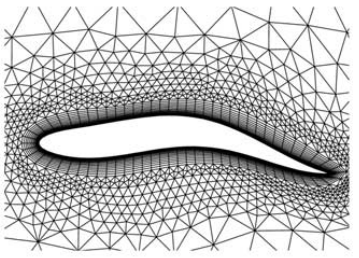
\includegraphics[scale=0.25]{dgm-movedmesh}
	}
	\caption{The DGM process}
\end{figure}

\end{frame}

\begin{frame}{Radial Basis Function (RBF) Interpolation}
In this method, global basis functions (which are radially symmetric) are used to represent the mesh deformation \cite{rbf}.

\begin{equation}
s(\mathbf{x}) = \sum_{i=1}^{N_b} \alpha_i \phi(||\mathbf{x}-\mathbf{x_{b}}_i||)
\end{equation}
Here, $\mathbf{x_{b}}_i$ is the position of the $i$th boundary node, $\alpha_i$ is the coefficient of the basis function $\phi_i = \phi(||\mathbf{x}-\mathbf{x_{b}}_i||)$, $s(\mathbf{x})$ is the displacement at point $\mathbf{x}$ in the domain.
\end{frame}

\begin{frame}{RBF interpolation}
We first need to calculate the coefficients of the RBFs by using the boundary displacement information. This involves solving a symmetric positive-definite system of equations for the coefficients $\alpha_i$.
\begin{equation}
s_{b_j}(\mathbf{x}) = \sum_{i=1}^{N_b} \alpha_i \phi(||\mathbf{x_{b}}_j-\mathbf{x_{b}}_i||) \quad \forall \, j \in \{1,2,...N_b \}
\end{equation}
Thus, a linear system needs to be solved for RBF interpolation, as opposed to DG-based methods.
\end{frame}

\begin{frame}{Delaunay graph mapping with radial basis functions}
Wang, Qin and Zhao combined the Delaunay graph mapping method with RBF interpolation to produce what they call the DG-RBF method \cite{dgrbf}.

This method is similar to the original DGM, except that the interpolation is done using RBFs instead of area coordinates. This gives much more control over the nature of interpolation.

For problems with severe rotational motion, rotation angles can also be interpolated along with displacements.
\end{frame}

\section{Comparison in case of large mesh deformation}
\begin{frame}[allowframebreaks]{Comparison}
All of the above methods were tested on a case of flap-rotation in a 3-component airfoil inviscid mesh. It was found that the methods of linear elasticity, DGM and RBF were effective enough to be considered. Though DG-RBF is claimed to be better than DGM, I have been unable to make it work even as well as DGM for this case.
\begin{itemize}
\item DGM was observed to be faster than the RBF method. The RBF method is, in turn, observed to be significantly faster than linear elasticity. 

This is expected: DGM has to solve no linear system - it only needs to construct a triangulation of the boundary points; RBF needs to solve a linear system of size $N_b \times N_b$, where $N_b$ is the number of boundary points; linear elasticity needs to solve a system of size $2N \times 2N$, where $N$ is the total number of nodes in the mesh. 

\item At about $60^\circ$ of rotation, mesh quality of DGM is worst, followed by linear elasticity, and RBF gives the best mesh quality (by visual inspection of the mesh). Linear elasticity does give somewhat better mesh quality away from the moving boundary, though.

\item Linear elasticity failed beyond an angle of $60^\circ$ CW, whereas RBF and DGM can go much beyond that. However, DGM fails for CCW angles of rotation, even as small as 10 to 15 degrees. Linear elasticity can go up to 30 degrees or so, while RBF did not produce invalid elements up to 40 degrees (possibly more).
\end{itemize}
\end{frame}

\begin{frame}{Deformed meshes}
\begin{figure}
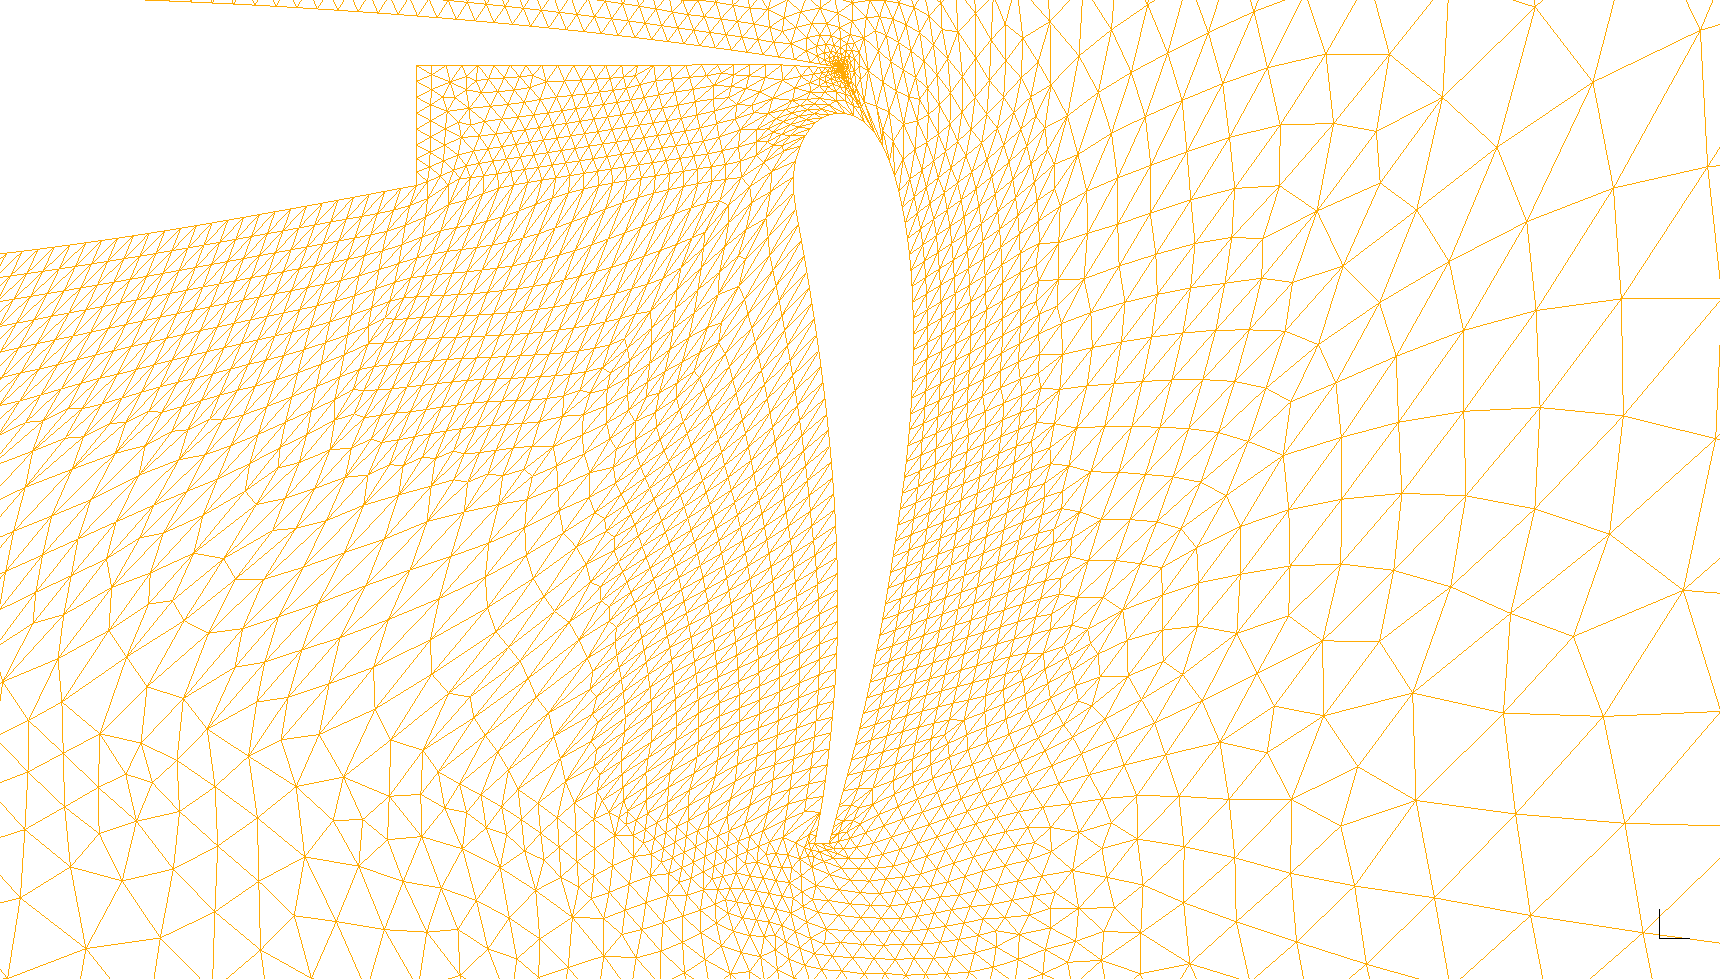
\includegraphics[scale=0.18]{movedwing-dgm--60-2}
\caption{DGM}
\end{figure}
\end{frame}

\begin{frame}{Deformed meshes}
\begin{figure}
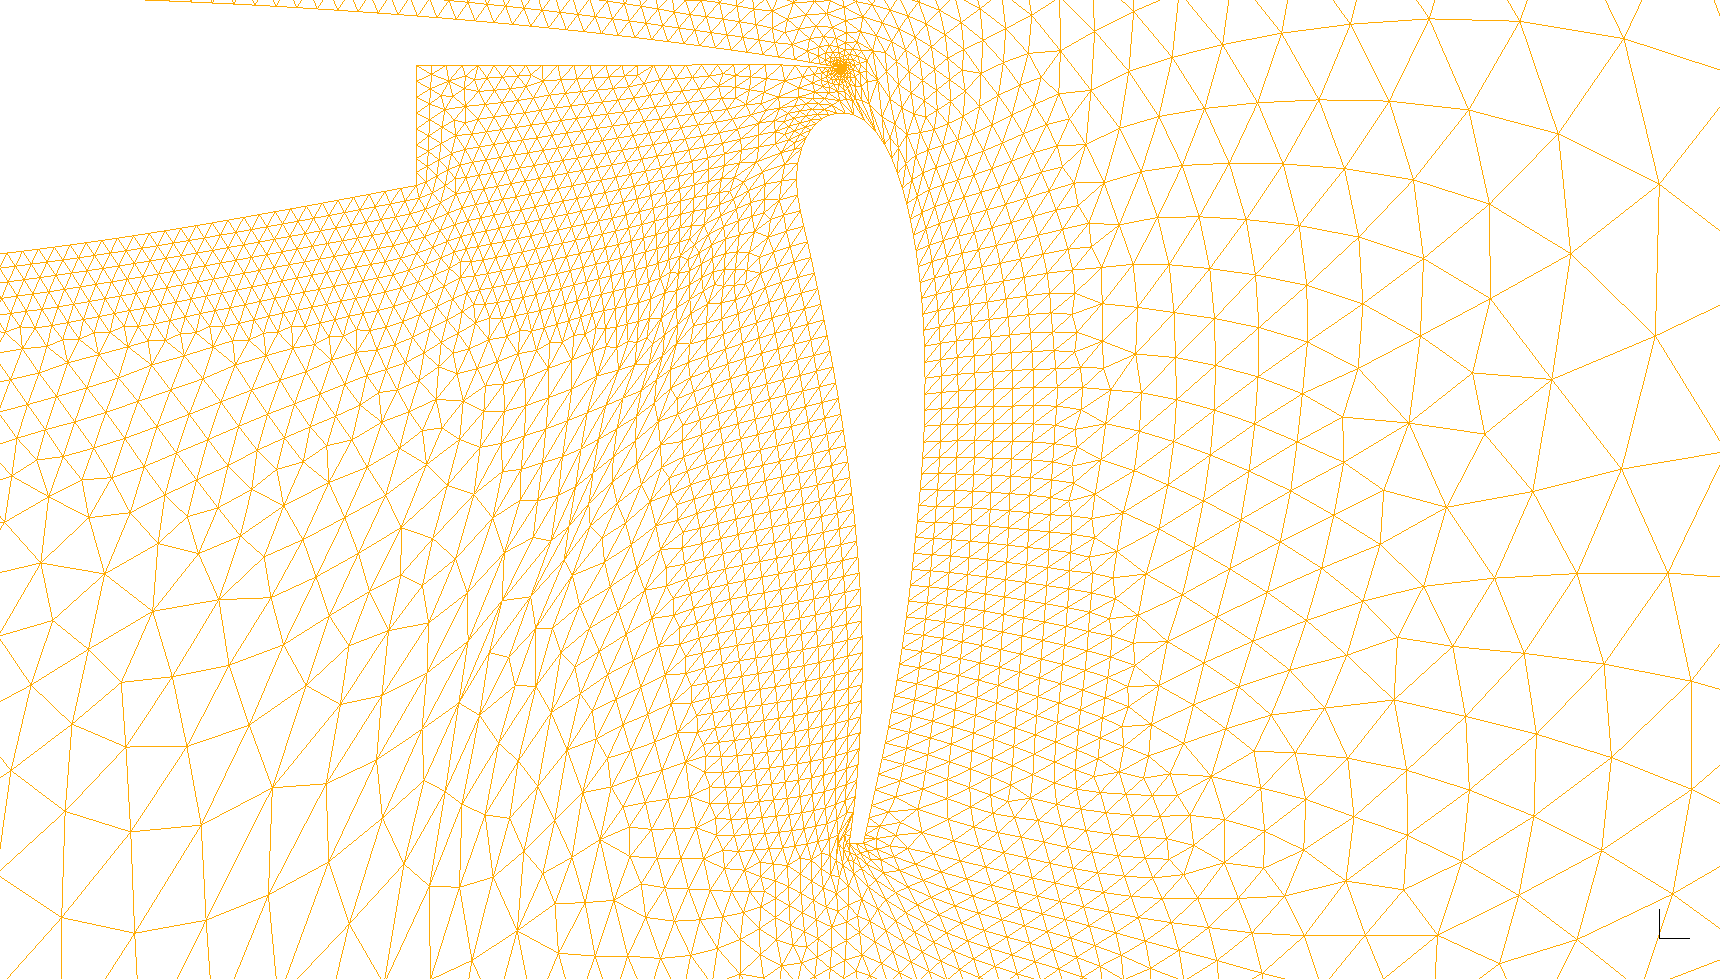
\includegraphics[scale=0.2]{movedwing-elast--60-2}
\caption{Linear elasticity}
\end{figure}
\end{frame}

\begin{frame}{Deformed meshes}
\begin{figure}
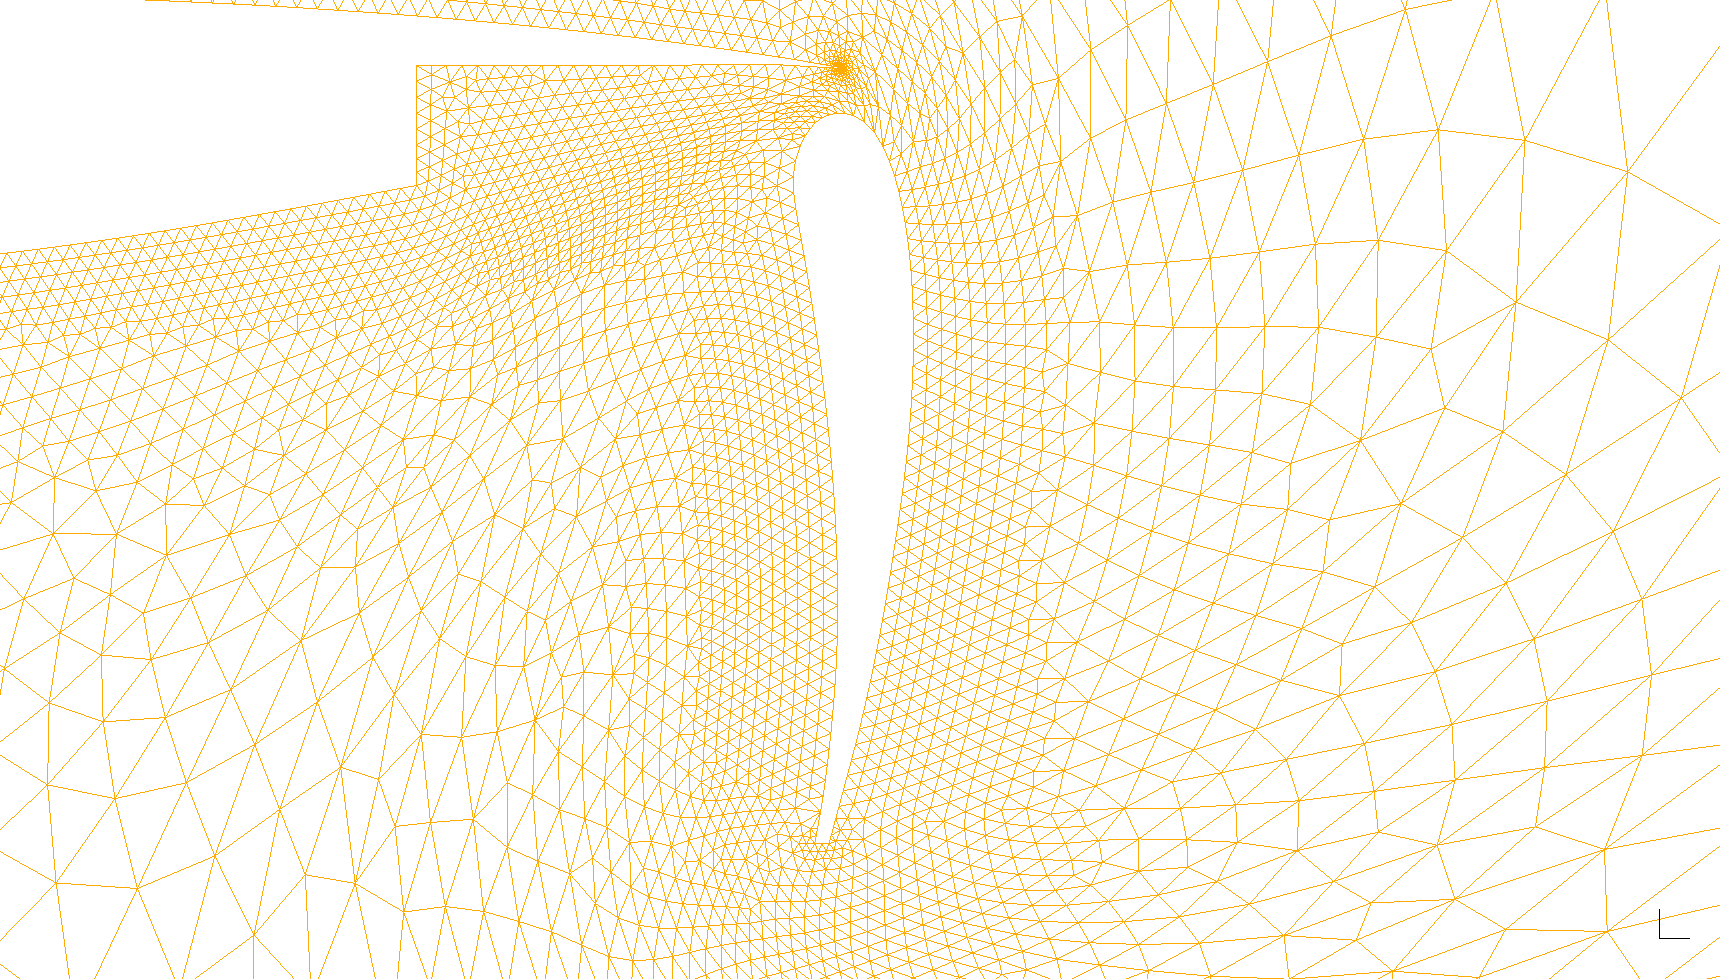
\includegraphics[scale=0.2]{movedwing-rbf--60-2}
\caption{RBF}
\end{figure}
\end{frame}


\begin{frame}{Deformed meshes}
\begin{figure}
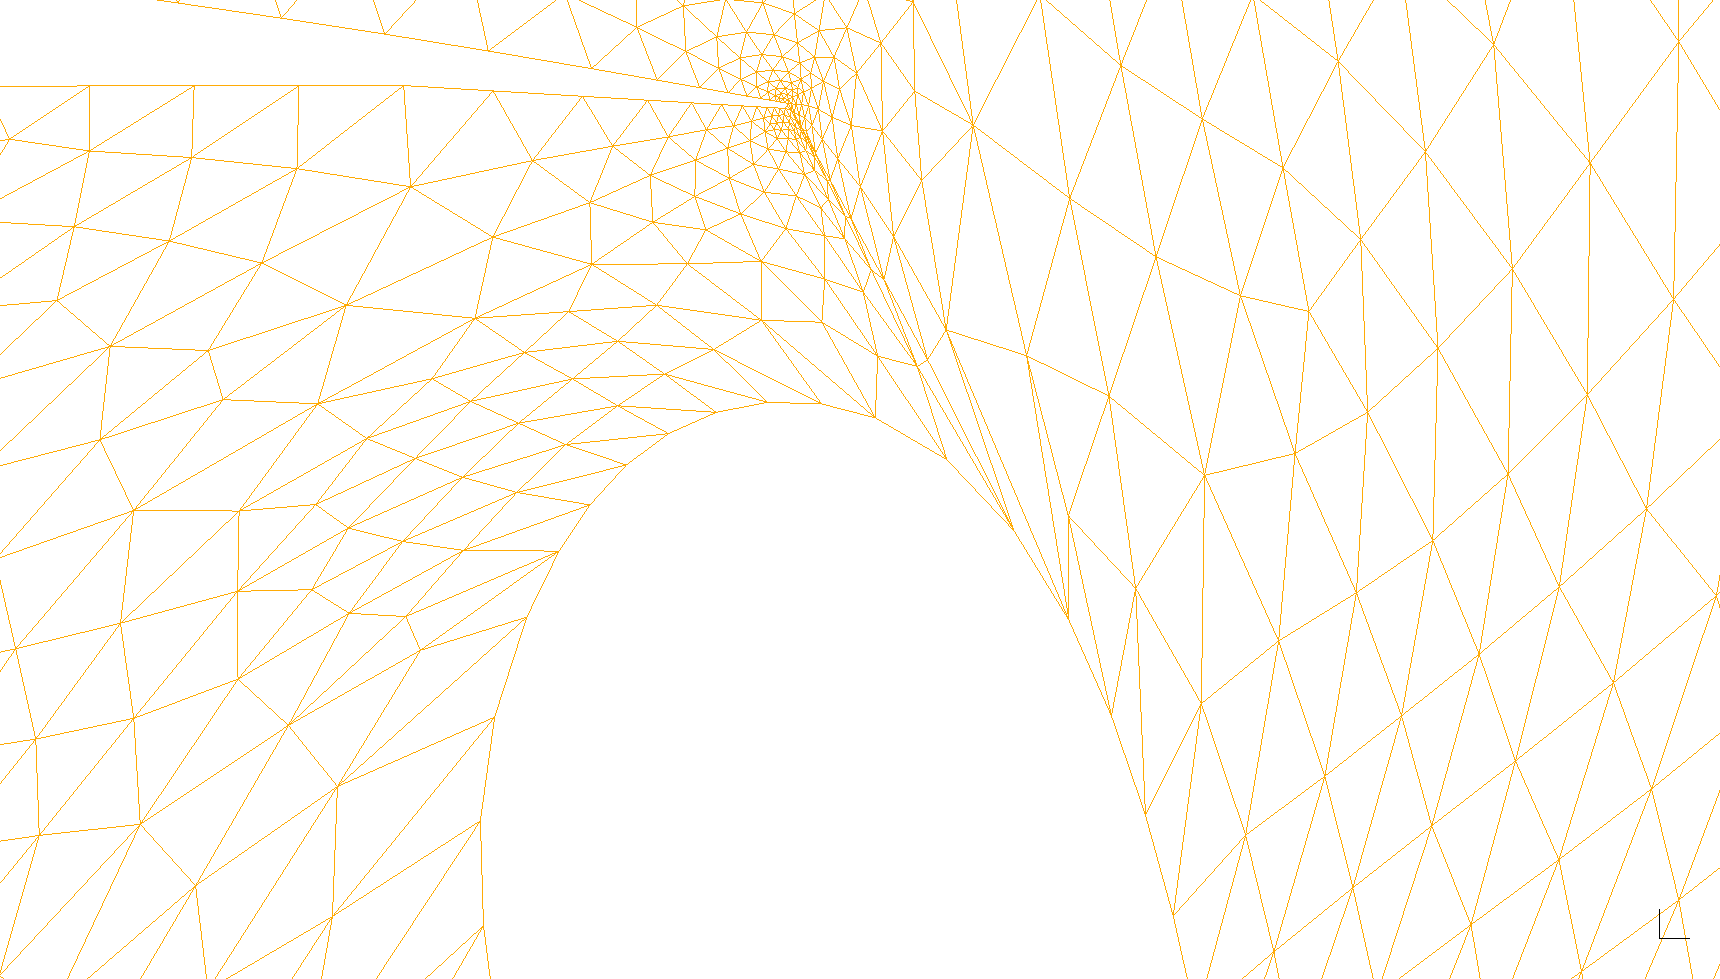
\includegraphics[scale=0.18]{movedwing-dgm--60}
\caption{DGM}
\end{figure}
\end{frame}

\begin{frame}{Deformed meshes}
\begin{figure}
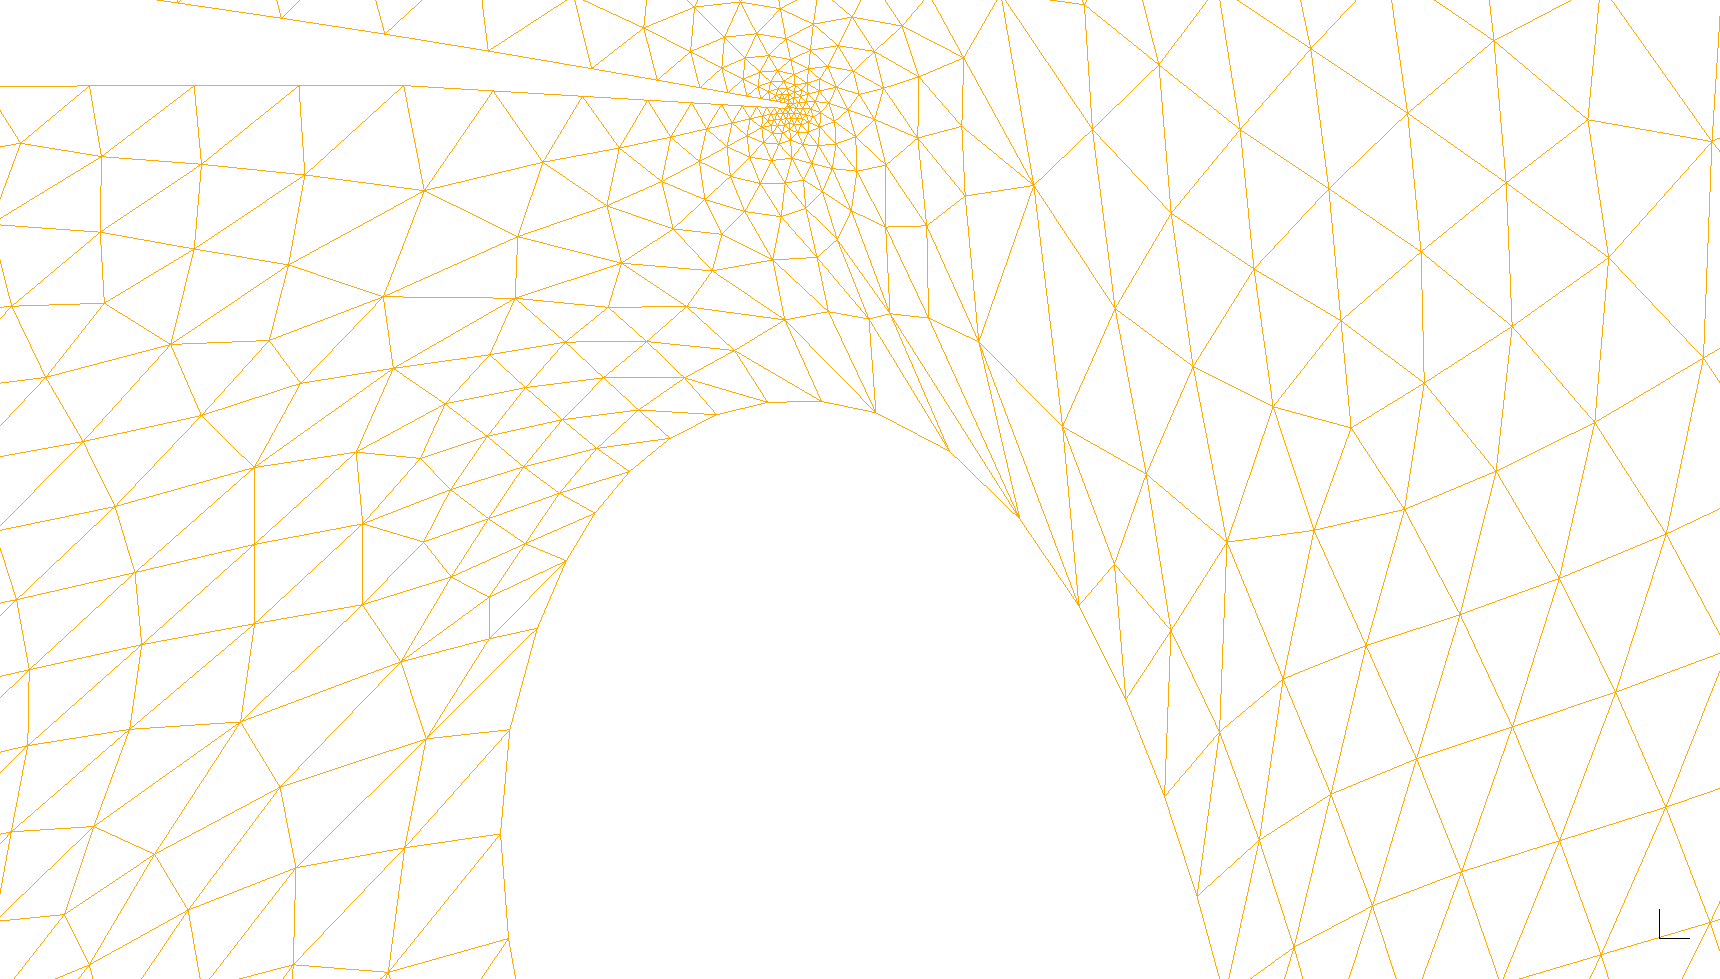
\includegraphics[scale=0.18]{movedwing-elast--60}
\caption{Linear elasticity}
\end{figure}
\end{frame}

\begin{frame}{Deformed meshes}
\begin{figure}
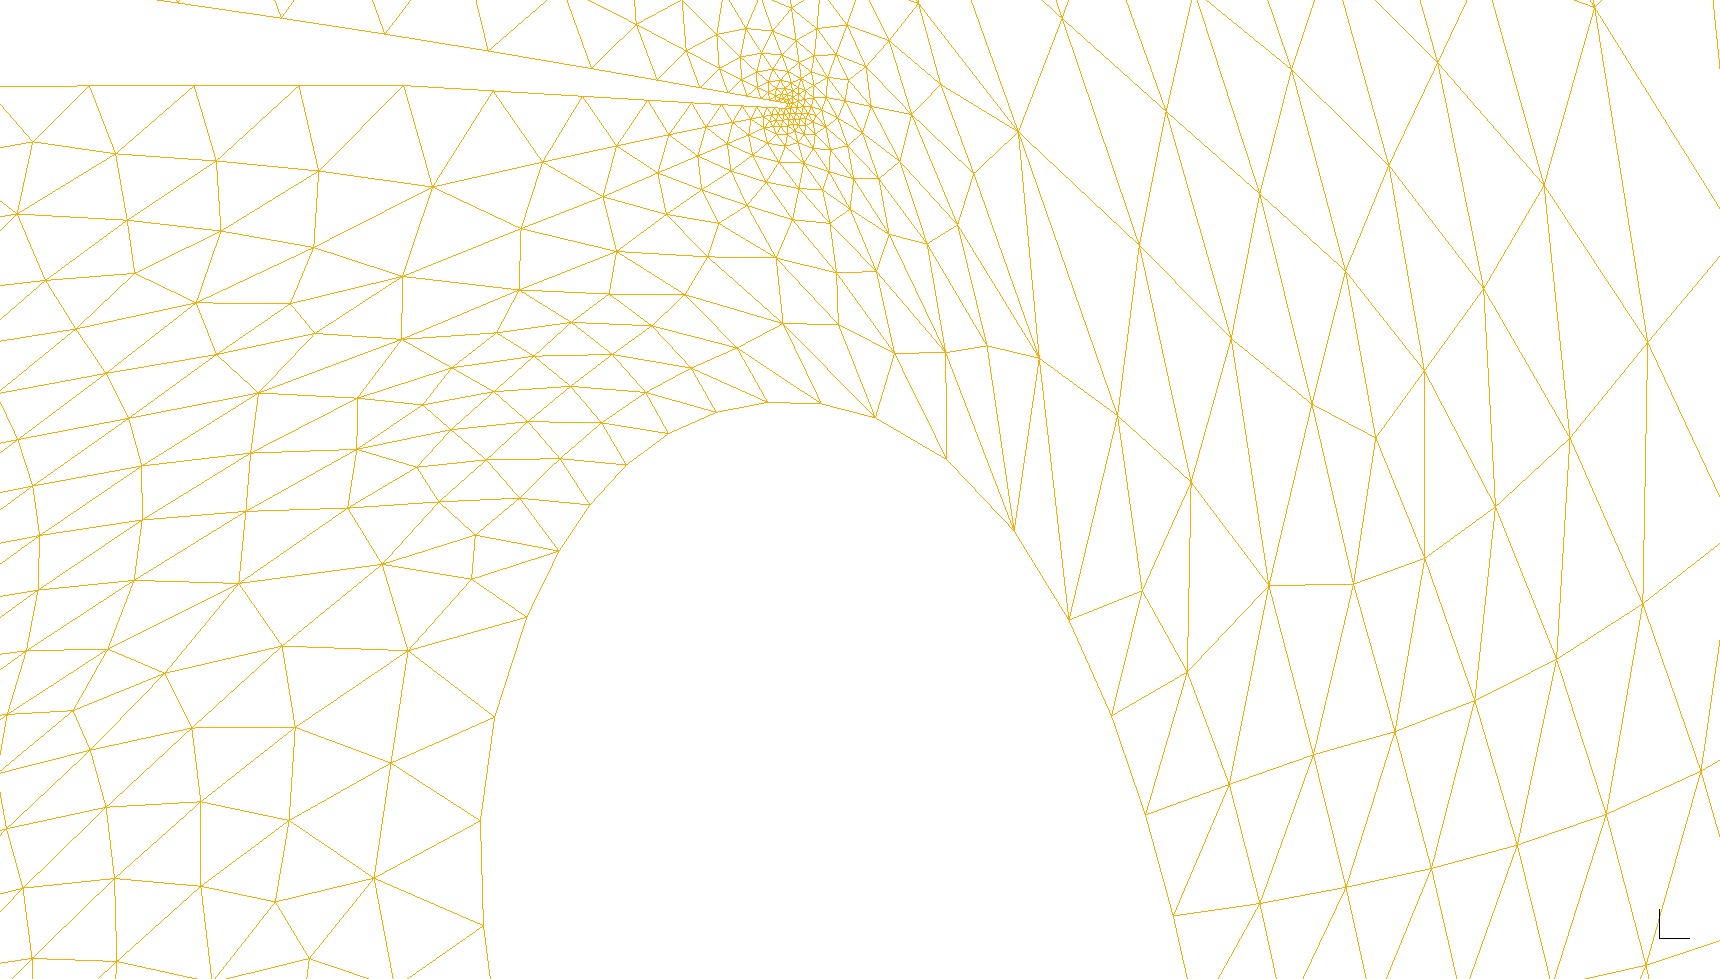
\includegraphics[scale=0.18]{movedwing-rbf--60}
\caption{RBF}
\end{figure}
\end{frame}

\section{Curved Mesh Generation}

\begin{frame}
If we only have boundary elements as high order, and move the boundary nodes to better conform to the true boundary, we may get invalid boundary elements.

Thus we need internal elements to be curved as well, and mesh movement methods can be used for this.

\begin{figure}
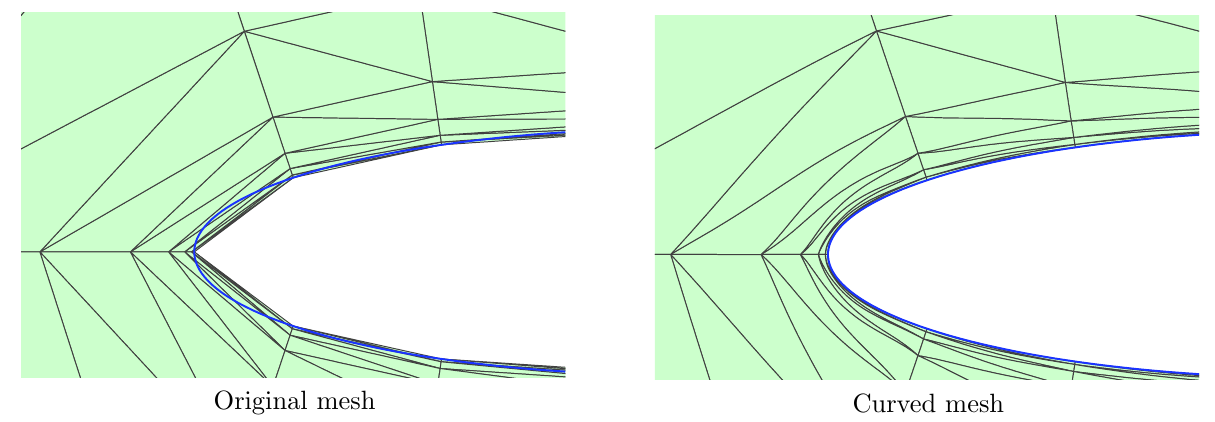
\includegraphics[scale=0.25]{curved-mesh-example}
\caption{Example of requirement of interior mesh curving, taken from \cite{perssonelast}.}
\end{figure}
\end{frame}

\begin{frame}{Curved Mesh Generation by Interpolation Methods}
I tried to generate a curved mesh for 2D bump using DGM and RBF methods.

The RBF method works very well (it would seem) with a minimum scaled Jacobian range of ~0.85 to 1.0, though I have not computed any skew (distortion) metric yet.

The DGM method, unfortunately, does not work due to the nature of this interpolation method - it is local in each Delaunay element, rather than global as in the case of RBF method.
\end{frame}

\section{Conclusion}
\begin{frame}
The next steps are to
\begin{itemize}
\item Write pre-processing code so that 3D curved meshes can be generated.
\item Write code to compute mesh-quality metrics.
\end{itemize}
\end{frame}

\begin{frame}[allowframebreaks]{References}
\bibliography{references}
\end{frame}

\end{document}